\section{Regression}

\subsection{Linear Regression}

In statistical modeling, regression analysis consists of a set of statistical processes and techniques for estimating the relationships between a dependent variable (often called the outcome or response variable, or a label in machine learning) and one or more error-free independent variables (often called regressors, predictors, covariates, explanatory variables or features). 

The goal of regression is then to predict the value of one or more continuous response variables $y$ given the values of a $m$-dimensional vector $\vec{x}$ of \emph{input} (features) variables. Usually we are given a training data set which contains a fixed number $N$ of observations $\{\vec{x_n}\}_{n=1,2,...,N}$ together with their corresponding outcome values $\{y_n\}$. The goal is then to predict the value of $y$ for a new given value of $\vec{x} \in \RR^{m}$. For instance, suppose we have a dataset giving the living areas, number of rooms, the district number location and prices of $50$ departments in Paris, France: \\

\begin{center}
\begin{tabular}{|c|c|c|c|}
	\hline
	Living Area (\si{\square\meter}) &  Number of Rooms &  District &  Price (\euro) \\
	\hline
	57.45  & 3  &  9  &  319000  \\
	47.93  & 2  & 15  &  220000  \\
	59.72  & 3  & 13  &  324000  \\
	72.85  & 4  &  1  &  411000  \\
	46.49  & 2  &  7  &  282000  \\
	46.49  & 2  &  9  &  242000  \\
	73.69  & 4  &  1  &  392000  \\
	61.51  & 3  & 12  &  328000  \\
	42.96  & 2  &  8  &  253000  \\
	58.14  & 3  & 11  &  327000  \\
	43.05  & 2  & 19  &  225000  \\
	43.01  & 2  & 17  &  245000  \\
	53.63  & 3  &  8  &  300000  \\
	21.30  & 1  &  3  &  136000  \\
	24.13  & 1  &  3  &  117000  \\
%	41.57  & 2  &  1  &  221000  \\
%	34.81  & 2  &  5  &  186000  \\
%	54.71  & 3  & 10  &  274000  \\
%	36.38  & 2  &  7  &  208000  \\
%	28.82  & 1  &  9  &  159000  \\
	$\vdots$ & $\vdots$ & $\vdots$ & $\vdots$ \\
\end{tabular}
\end{center}

We can plot this data to observe the Price according to the Living Area:


\begin{center}
	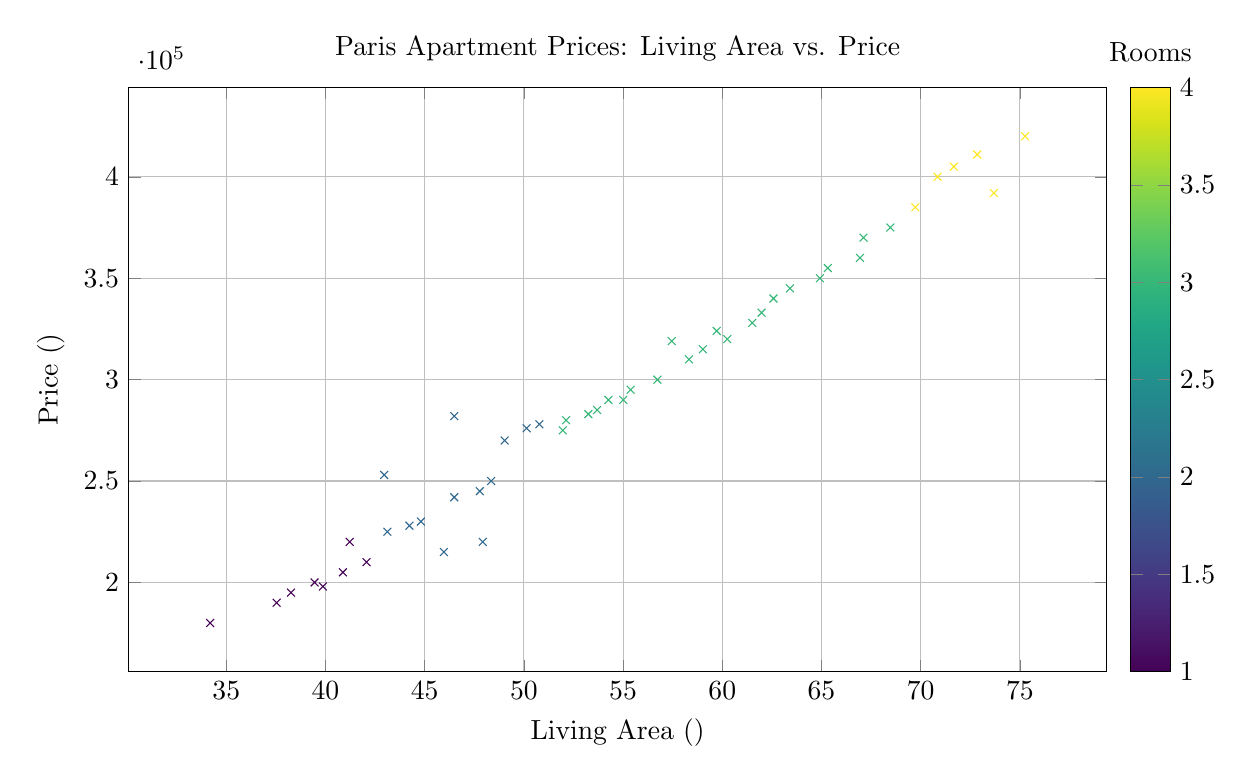
\begin{tikzpicture}
		\begin{axis}[
			width=14cm,  % Increase width
			height=9cm, % Increase height
			title={Paris Apartment Prices: Living Area vs. Price},
			xlabel={Living Area (\si{\square\meter})},
			ylabel={Price (\euro)},
			grid=major,
			colorbar,
			colormap/viridis,
			point meta=min,
			point meta=max,
			scatter/use mapped color={draw=mapped color, fill=mapped color},
			scatter,
			colorbar style={title=Rooms},
			%yticklabel style={/pgf/number format/fixed} % Ensure regular number formatting
			]
			\addplot[
			scatter, only marks,
			mark=x, % Change marker to x
			mark size=2pt,
			scatter src=explicit
			]
			table [meta=Number_of_Rooms] {
				Living_Area Price Number_of_Rooms
				57.45 319000 3
				47.93 220000 2
				59.72 324000 3
				72.85 411000 4
				46.49 282000 2
				46.49 242000 2
				73.69 392000 4
				61.51 328000 3
				42.96 253000 2
				65.32 355000 3
				54.26 290000 3
				50.14 276000 2
				71.67 405000 4
				34.19 180000 1
				45.97 215000 2
				49.03 270000 2
				75.26 420000 4
				39.45 200000 1
				62.58 340000 3
				58.32 310000 3
				41.22 220000 1
				37.54 190000 1
				55.38 295000 3
				66.94 360000 3
				44.81 230000 2
				53.69 285000 3
				67.12 370000 3
				60.25 320000 3
				56.73 300000 3
				38.26 195000 1
				70.85 400000 4
				63.41 345000 3
				43.12 225000 2
				47.78 245000 2
				48.35 250000 2
				64.92 350000 3
				52.13 280000 3
				59.02 315000 3
				42.07 210000 1
				40.88 205000 1
				55.01 290000 3
				68.47 375000 3
				51.96 275000 3
				39.87 198000 1
				44.23 228000 2
				50.78 278000 2
				53.25 283000 3
				61.98 333000 3
				69.73 385000 4
			};
		\end{axis}
	\end{tikzpicture}
\end{center}

%We can also plot the Price against the number of rooms and District: 
%
%\begin{center}
%	\begin{tikzpicture}
%		\begin{axis}[
%			width=14cm,  % Increase width
%			height=9cm, % Increase height
%			title={Paris Apartment Prices: Number of Rooms vs. Price},
%			xlabel={Number of Rooms},
%			ylabel={Price (€)},
%			grid=major,
%			scatter,
%			yticklabel style={/pgf/number format/fixed} % Ensure regular number formatting
%			]
%			\addplot[
%			scatter, only marks,
%			mark=x, % Change marker to x
%			mark size=3pt
%			]
%			table {
%				Number_of_Rooms Price
%				3 319000
%				2 220000
%				3 324000
%				4 411000
%				2 282000
%				2 242000
%				4 392000
%				3 328000
%				2 253000
%				3 355000
%				3 290000
%				2 276000
%				4 405000
%				1 180000
%				2 215000
%				2 270000
%				4 420000
%				1 200000
%				3 340000
%				3 310000
%				1 220000
%				1 190000
%				3 295000
%				3 360000
%				2 230000
%				3 285000
%				3 370000
%				3 320000
%				3 300000
%				1 195000
%				4 400000
%				3 345000
%				2 225000
%				2 245000
%				2 250000
%				3 350000
%				3 280000
%				3 315000
%				1 210000
%				1 205000
%				3 290000
%				3 375000
%				3 275000
%				1 198000
%				2 228000
%				2 278000
%				3 283000
%				3 333000
%				4 385000
%			};
%		\end{axis}
%	\end{tikzpicture}
%\end{center}
%
%\begin{center}
%	\begin{tikzpicture}
%		\begin{axis}[
%			title={Paris Apartment Prices: District vs. Price},
%			xlabel={District Number},
%			ylabel={Price (€)},
%			grid=major,
%			scatter,
%			yticklabel style={/pgf/number format/fixed} % Ensure regular number formatting
%			]
%			\addplot[
%			scatter, only marks,
%			mark=x, % Change marker to x
%			mark size=3pt
%			]
%			table {
%				District Price
%				9 319000
%				15 220000
%				13 324000
%				1 411000
%				7 282000
%				9 242000
%				1 392000
%				12 328000
%				8 253000
%				11 355000
%				19 290000
%				17 276000
%				8 405000
%				3 180000
%				3 215000
%				1 270000
%				5 420000
%				10 200000
%				7 340000
%				9 310000
%				9 220000
%				6 190000
%				4 295000
%				2 360000
%				5 230000
%				8 285000
%				18 370000
%				16 320000
%				14 300000
%				10 195000
%				2 400000
%				20 345000
%				17 225000
%				12 245000
%				11 250000
%				13 350000
%				6 280000
%				15 315000
%				4 210000
%				19 205000
%				5 290000
%				16 375000
%				10 275000
%				14 198000
%				7 228000
%				9 278000
%				20 283000
%				3 333000
%				8 385000
%			};
%		\end{axis}
%	\end{tikzpicture}
%\end{center}

Given data like this, we would like to learn to predict the prices of other apartments in Paris, as a function of the input features $(\text{Living Area},\text{Rooms},\text{District})$. Let us first introduce some notation: We set $\vec{x}^{(i)} = (x_1^{(i)},x_2^{(i)},x_3^{(i)})$ to be the vector in $\RR^3$ whose entries correspond to the features $(\text{Living Area},\text{Rooms},\text{District})$ of the $i$-th apartment in the training set (see Table). For instance, according to the Table 
\[\vec{x}^{(1)}= (57.45, 3, 9)\]

Let $y^{(i)}$ be the output or \emph{target} variable that we are trying to predict; in our case it represents the Price. For instance $y^{(1)} = 319000$. The dataset that we will use to learn consist then of the list of $N=50$ training examples: 
\[\left\{ \left( \vec{x}^{(i)}, y^{(i)} \right) \ : \ i=1,2,...,N \right\}\]
This last list will be then called \emph{training set}. 

\begin{remark}
	In general when constructing a learning problem we have freedom over which features to use so one may decide to collect more data and include other features. We will say more about feature selection later. 
\end{remark}

To achieve the goal of predicting the value of $y$ for new given vectors of $\vec{x} \in \RR^m$, we will formulate a function $y(\vec{x},\vec{w})$ whose values are the predictions for new inputs $\vec{x}$, and where $\vec{w}$ represents a vector of parameters that will be learned from the training set. 

The simplest model for the function $y(\vec{x},\vec{w})$ is the one that consist of a linear combination of the inputs: 

\begin{equation}\label{Eq.Sec.Lin.Reg.1}
	y(\vec{x},\vec{w}) = w_0 + w_1x_1 + \cdots + w_m x_m
\end{equation}

\begin{remark}
	The parameter $w_0$ is usually called a \emph{bias parameter}. The key property of this model is that it is a linear function of the parameters $w_0,...,w_m$ and also of the input variables $x_1,...,x_m$. 
\end{remark}


\subsubsection{Non linear models}

The class of linear models defined by \cref{Eq.Sec.Lin.Reg.1} can be easily extended by considering linear combinations of non-linear functions of the input features $\vec{x}$. More precisely, suppose $\phi_0,...,\phi_m : \RR^m \lto \RR$ are a collection of \emph{basis} functions. Then, we can consider models of the form: 

\[ y(\vec{x},\vec{w}) = w_0 + \sum_{i=1}^{m}w_i\phi_i(\vec{x})\]
For convenience we will set $\phi_0$ to be the constant function $1$ so that the last equation becomes: 

\begin{equation}\label{Eq.Sec.Lin.Reg.2}
	y(\vec{x},\vec{w}) = \sum_{i=0}^{m}w_i\phi_i(\vec{x}) = \vec{w}^T\phi(x)
\end{equation}
where $\vec{w} = (w_0,...,w_m)^T$ and $\phi = (\phi_0,...,\phi_m)^T$.

\begin{remark}
	Models like \cref{Eq.Sec.Lin.Reg.2} are called \emph{linear models} because they are linear in the parameters $\vec{w}$, nevertheless the model $y(\vec{w},\vec{x})$ can be a non-linear function of the inputs $\vec{x}$ (it suffices to consider non-linear basis functions). Moreover, notice that if each $\phi_j$ is defined as the projection onto the $j$-th coordinate then \cref{Eq.Sec.Lin.Reg.2} recovers \cref{Eq.Sec.Lin.Reg.1}. 
\end{remark}

Before deep learning it was common practice in classical machine learning to use some form of fixed pre-processing of the input variables x, also known as \emph{feature extraction}, expressed in terms of a set of basis functions. The goal was to find a powerful set of basis functions that the resulting learning task could be solved using a simple network model. This is very difficult task. Deep Learning avoids this problem by learning the required nonlinear transformations of
the data from the data set itself. This turns out to be very useful for problems about image recognition. 

In the following table we provide a list of some common useful choices of the basis functions (assuming a single feature $x$): 

	% Please add the following required packages to your document preamble:
	% \usepackage{multirow}
	\begin{table}[ht!]
		\centering
		\begin{tabular}{ccc}
			\hline
			\begin{tabular}[c]{@{}c@{}}Basis functions\\ $\phi_j(x)$\end{tabular} &
			\begin{tabular}[c]{@{}c@{}}Model equation\\ $y(x,\vec{w})$\end{tabular} &
			Model nature \\ \hline
			\multirow{2}{*}{$x^j$} &
			\multirow{2}{*}{$w_0 + w_1x + w_2x^2 + \cdots +w_mx^m$} &
			\multirow{2}{*}{Polynomial} \\
			&  &  \\ \hline
			\multirow{2}{*}{$\exp\left( - \frac{(x-\mu_j)^2}{2s^2}\right)$} &
			\multirow{2}{*}{$ \sum w_i \exp\left( - \frac{(x-\mu_j)^2}{2s^2}\right)$} &
			\multirow{2}{*}{Gaussian basis functions} \\
			&  &  \\ \hline
			\multirow{2}{*}{$\sigma\left( \frac{x- \mu_j}{s}\right)$} &
			\multirow{2}{*}{$\sum w_i \sigma\left( \frac{x-\mu_i}{s} \right)$} &
			\multirow{2}{*}{Sigmoidal basis functions} \\
			&  &  \\ \hline
		\end{tabular}
	\end{table}
where $\sigma$ denotes the sigmoid function defined by 
\[ \sigma(z) = \frac{1}{1+ \exp(-z)}\]


\subsubsection{Maximum likelihood}

There are different ways to estimate the parameters $\vec{w}$ for a given model $y(\vec{x},\vec{w})$ using the dataset $\left\{ \left( \vec{x}^{(i)}, y^{(i)} \right) \ : \ i=1,2,...,N \right\}$. Perhaps the most common method consist of finding the parameters $\vec{w}$ that maximize a certain function called \emph{likelihood function}. To derive such function we must make some assumptions about the relation between the target variables $y^{(i)}$ and the inputs $\vec{x}^{(i)}$.

Let us then assume that the target variable $y$ is given by a deterministic function as in \ref{Eq.Sec.Lin.Reg.2} $y(\vec{x},\vec{w})$ with some additive Gaussian noise. This means that the target values and the inputs are related by an equation

\begin{equation}\label{Eq.Sec.Lin.Reg.3} 
y = y(\vec{x},\vec{w}) + \epsilon 
\end{equation}
where $\epsilon$ is a random variable that captures either unmodeled effects (\eg missing important features) or random noise. We assume further that $\epsilon$ is a zero-mean Gaussian with variance $\sigma^2$. We can write this last assumption as $\epsilon \simeq \mathcal{N}(0,\sigma^2)$. Therefore, the probability density of $\epsilon$ is given by 

\[ p(\epsilon) = \frac{1}{\sqrt{2\pi}\sigma}\exp\left( - \frac{\epsilon^2}{2\sigma^2}\right)\]
By substituting in \ref{Eq.Sec.Lin.Reg.3} we then get $p(y| \vec{x}; \vec{w}, \sigma) \simeq \mathcal{N}(y(\vec{x},\vec{w}, \sigma))$. In other words,  

\begin{equation}
	p(y| \vec{x}; \vec{w}, \sigma) = \frac{1}{\sqrt{2\pi}\sigma}\exp\left( - \frac{(y-\vec{w}^T\phi(\vec{x}))^2}{2\sigma^2}\right)
\end{equation}
\stnote{There's an error here in this matrix, one has to include phi}
Finally we can then consider the \emph{design matrix} whose rows correspond to the vectors $\vec{x}^{(i)}$ in the dataset together with the vector or target values $\vec{y}$, \ie, 

\[ X = \begin{bmatrix}
	x_{1}^{(1)} & x_{2}^{(1)} & x_{3}^{(1)} & \dots  & x_{m}^{(1)} \\
	x_{1}^{(2)} & x_{2}^{(2)} & x_{3}^{(2)} & \dots  & x_{m}^{(2)} \\
	\vdots & \vdots & \vdots & \ddots & \vdots \\
	x_{1}^{(N)} & x_{2}^{(N)} & x_{3}^{(N)} & \dots  & x_{m}^{(N)}
\end{bmatrix}_{Nxm} \quad \vec{y} = \begin{bmatrix}
y^{(1)} \\
y^{(2)} \\ 
\ddots \\
y^{(N)}
\end{bmatrix}\]


\begin{remark}
	Once we start using our dataset we are working under the assumption that each $y^{(i)}$ satisfies a relation as in \ref{Eq.Sec.Lin.Reg.3} and moreover these of the $\epsilon^{(i)}$ are themselves independent (and hence also the $y^{(i)}$'s given the $\vec{x}^{(i)}$'s).
\end{remark}

From the last assumption we obtain an expression for the likelihood function: 

\begin{equation}
	L(\vec{w}) = L(\vec{w}; X,\vec{y}) = p (\vec{y}| X, \vec{w}, \sigma^2) = \prod_{i=1}^{N} p(y^{(i)}| \vec{x}^{(i)},\vec{w},\sigma)
\end{equation}

The principle of \emph{maximum likelihood} implies that we should choose the parameters $\vec{w}$ so that the data has the highest possible probability. In other words, we should choose $\vec{w}$ so that the maximum likelihood function $L(\vec{w})$ is maximum. To simplify calculations we can, equivalently, maximize the \emph{log likelihood} $\ell(\vec{w}) = \ln (L(\vec{w}))$. A simple calculation shows that

\begin{align}
	\ell(\vec{w}) &= \sum_{i=1}^N \ln \left( \frac{1}{\sqrt{2\pi}\sigma} \exp\left(-\frac{(y^{(i)}- \vec{w}^T\phi(\vec{x}^{(i)}))^2}{2\sigma^2}\right)\right) \\ &= -\frac{N}{2}\ln(2\pi) - \frac{N}{2}\ln(\sigma^2) - \frac{1}{\sigma^2}\cdot \underbrace{\frac{1}{2}\sum_{i=1}^{N} (y^{(i)} - \vec{w}^T\phi(\vec{x}^{(i)}) )^2}_{J(\vec{w})}
\end{align}

The first two quantities in the last equality are constant and therefore, maximizing the log likelihood $\ell(\vec{w})$ is equivalent to minimizing the \emph{sum-of-squares error function}, also called the \emph{cost function} $J(\vec{w})$: 

\begin{equation}\label{Eq.Sec.Lin.Reg.4}
	J(\vec{w}) = \frac{1}{2}\sum_{i=1}^{N} (y^{(i)} - \vec{w}^T\phi(\vec{x}^{(i)}) )^2
\end{equation}

We will observe two ways of minimizing the cost function $J$. 

\subsubsection{Gradient Descent and LMS algorithm}

Recall we want to find the parameters $\vec{w}$ so that the cost function $J(\vec{w})$ is minimized. To do this we can use the \emph{gradient descent} algorithm. The idea is to start with an initial guess, say, $\vec{w} = (w_0,w_1,...,w_m)$ and then iteratively update the parameters using the following rule: 

\begin{equation}\label{Eq.Sec.Lin.Reg.5}
	\vec{w} \leftarrow \vec{w} - \eta \nabla J(\vec{w})
\end{equation} 
where $\eta$ is a (usually small) positive number called the \emph{learning rate} and $\nabla J(\vec{w})$ is the gradient of the cost function $J(\vec{w})$. The gradient is a vector whose components are given by the partial derivatives of $J$ with respect to each parameter $w_j$:
\begin{equation}\label{Eq.Sec.Lin.Reg.6}
	\nabla J(\vec{w}) = \begin{bmatrix}
	\frac{\partial J}{\partial w_0} \\[0.7em]
	\frac{\partial J}{\partial w_1} \\[0.7em]
	\vdots \\
	\frac{\partial J}{\partial w_m}
	\end{bmatrix} = -\begin{bmatrix} 
	\sum_{i=1}^{N} (y^{(i)} - \vec{w}^T\phi(\vec{x}^{(i)}))\phi_0(\vec{x}^{(i)}) \\[0.7em]
	\sum_{i=1}^{N} (y^{(i)} - \vec{w}^T\phi(\vec{x}^{(i)}))\phi_1(\vec{x}^{(i)}) \\[0.7em]
	\vdots \\[0.7em]
	\sum_{i=1}^{N} (y^{(i)} - \vec{w}^T\phi(\vec{x}^{(i)}))\phi_m (\vec{x}^{(i)})
	\end{bmatrix}
\end{equation}

By replacing in \cref{Eq.Sec.Lin.Reg.5} and grouping all coordinates we obtain the following update vector rule for the parameters:

\begin{equation}
	\vec{w} \leftarrow \vec{w} + \eta \cdot \sum_{i=1}^{N} (y^{(i)} - \vec{w}^T\phi(\vec{x}^{(i)}))\phi(\vec{x}^{(i)}) 
\end{equation}

This rule is called the \emph{Least Mean Squares update rule}, sometimes also refered as (LMS) algorithm. The LMS algorithm is a stochastic gradient descent algorithm that updates the parameters $\vec{w}$ using the gradient of the cost function $J(\vec{w})$ at each iteration. The learning rate $\eta$ controls the step size of the update and can be adjusted to improve convergence. The full pseudo code for the LMS algorithm reads as follows: 

\begin{algorithm}[H]
	\caption{Least Mean Squares (LMS) Algorithm}
\begin{algorithmic}[1]
	\Require Training set $\{(\vec{x}^{(i)}, y^{(i)})\}_{i=1}^N$, learning rate $\eta$
	\Require Feature functions $\phi_j$, $j=0,1,\ldots,m$
	\State Initialize $\vec{w} \leftarrow \vec{0}$ or random values
	\Repeat
		\State $\vec{w} \leftarrow \vec{w} + \eta \sum_{i=1}^N (y^{(i)} - \vec{w}^T\phi(\vec{x}^{(i)}))\phi(\vec{x}^{(i)})$
	\Until{convergence or maximum iterations}
	\Return $\vec{w}$
\end{algorithmic}
\end{algorithm}


\begin{remark}
	This method is called \emph{batch gradient descent} because it uses the entire training set to compute the gradient at each iteration. In practice, we can also use \emph{stochastic gradient descent} (SGD) which updates the parameters using only one training example at a time. This is done by replacing the sum in \cref{Eq.Sec.Lin.Reg.5} by a single term $(y^{(i)} - \vec{w}^T\phi(\vec{x}^{(i)}))\phi(\vec{x}^{(i)})$ and iterate over each $i$. The SGD algorithm is usually faster than batch gradient descent and can be used for large datasets. 
\end{remark}

Finally notice also that the LMS algorithm is a special case of the more general \emph{gradient descent} algorithm. The main difference is that in the LMS algorithm we use the gradient of the cost function $J(\vec{w})$ to update the parameters $\vec{w}$, while in gradient descent we can use any function to update the parameters. In general gradient descent is susceptible to capture local minima of a function, while the LMS algorithm will capture one global minimum. This is because the cost function $J(\vec{w})$ is a convex function, which means that it has only one global minimum. In other words the LMS will always converge to the same solution regardless of the initial guess $\vec{w}$. 

\subsubsection{The Normal Equations}
The LMS algorithm is a very powerful method to minimize the cost function $J(\vec{w})$ but it can be slow to converge. In some cases, we can find the optimal solution for the parameters $\vec{w}$ in closed form. This is done by setting the gradient of the cost function $J(\vec{w})$ to zero and solving for $\vec{w}$. This gives us the so-called \emph{normal equations}:


\subsection{Python Implementation}

This section is dedicated to the implementation in python of the LMS algorithm via some problems and exercises taken from Andrew Ng CS229 course at Stanford University. We will use the \texttt{numpy} library which is a powerful library for numerical computing in Python, and the \texttt{pandas} library, a powerful library for data manipulation and analysis. We will also use the \texttt{matplotlib} library to plot the data and the results. In some other problems we will use the \texttt{scikit-learn} library which is a powerful library for machine learning in Python. These notes will contain the main functions and routines in Python. Additional code used to generate the figures and plots will be provided in the \faFolderOpen \texttt{Implementations} folder of the course repository. 

\subsubsection{Cost, Gradient and Gradient Descent}

\subsubsection*{Cost function}
Let us first implement a function that computes the cost function. Remember that the cost function is given by:	

\begin{equation}\label{Eq.Sec.Lin.Reg.7}
	J(\vec{w}) = \frac{1}{2}\sum_{i=1}^{N} (y^{(i)} - \vec{w}^T\phi(\vec{x}^{(i)}) )^2
\end{equation}	
we will assume that the basis functions $\phi_J$ are given by projections onto the $j$-th coordinate, \ie $\phi_j(\vec{x}) = x_j$. So that 

\[ \phi(\vec{x}^{(i)}) = \begin{bmatrix}
    1 & x_1^{(i)} & x_2^{(i)} & \cdots & x_m^{(i)}
\end{bmatrix}^{T} \]
In this case we can write the cost function as in \cref{Eq.Sec.Lin.Reg.1} as follows:

\begin{equation}\label{Eq.Sec.Lin.Reg.8}
	J(\vec{w}) = \frac{1}{2}\sum_{i=1}^{N} (y^{(i)} - \vec{w}^T \vec{x}^{(i)})^2
\end{equation}
where $x_0^{(i)}=1$ for all $i=1,...,N$. The code to compute the cost function for a single training example $\vec{x}$ and target value $y$ is then given by: 

\script{Classification}{utils.py}{compute_cost}[caption={Compute cost}, label={code:compute_cost}]

Along all these notes the common conventions and practices will be to use vectorized or Linear algebra notation. In the last code snippet, we start by append to the left a column of ones to the data matrix $X$. This is done to include the bias term $w_0$ in the model. Next we ensure that both the weights vector $\vec{w}$ and the outputs vector $\vec{y}$ are both seen as column vectors. The \texttt{{compute\_cost}} function takes $\vec{w}$ and $\vec{y}$ as 1D numpy arrays which are not the same as $Nx1$ and $m+1 x 1$ vectors. Finally we can compute the cost function by simply computing the vector difference \texttt{y - X@w}: 

\[ 
\begin{bmatrix} y^{(1)} \\ y^{(2)} \\ \vdots \\ y^{(N)}\end{bmatrix} - \begin{bmatrix}  
	1 & x_{1}^{(1)} & x_{2}^{(1)} & x_{3}^{(1)} & \dots  & x_{m}^{(1)} \\
	1 & x_{1}^{(2)} & x_{2}^{(2)} & x_{3}^{(2)} & \dots  & x_{m}^{(2)} \\
	\vdots & \vdots & \vdots & \vdots & \ddots & \vdots \\
	1 & x_{1}^{(N)} & x_{2}^{(N)} & x_{3}^{(N)} & \dots  & x_{m}^{(N)}
\end{bmatrix} \cdot \begin{bmatrix} w_0 \\ w_1 \\ \vdots \\ w_m \end{bmatrix} 
\]

Finally, the function simply uses the \texttt{np.sum} function to compute the sum of the squares of the differences. The \texttt{np.sum} function is a vectorized function that computes the sum of all the elements of an array much faster than a for loop.  

\subsubsection*{Gradient}
The next step is to implement the gradient descent algorithm. Recall that we have to update the parameters $\vec{w}$ using the gradient of the cost function $J(\vec{w})$. First, we create a function to compute the gradient:

\script{Classification}{utils.py}{compute_gradient}[caption={Compute Gradient}, label={code:compute_gradient}]

\begin{remark}
	The expression in line 17 of the code snippet is a vectorized version of the expression in \cref{Eq.Sec.Lin.Reg.6}. Formally we have a matrix product of $(\vec{y}- X\cdot \vec{w})^T$ with $X$ . The former expression is a $1xN$ vector and the latter is a $Nx(m+1)$ matrix.  The result is a $1x(m+1)$ vector containing the partial derivatives of the cost function with respect to each parameter $w_j$ or in other words, the gradient of the cost function.
\end{remark}

\subsubsection*{LMS algorithm} 
Finally we proceed to implement the LMS algorithm using gradient descent to minimize the sum-of-squares error function. We will use the \texttt{compute\_cost} and \texttt{compute\_gradient} functions to compute the cost and the gradient at each iteration. 
\script{Classification}{utils.py}{gradient_descent}[caption={Gradient Descent}, label={code:gradient_descent}]

\begin{observation}
It is common practice to consider an average cost function, \ie, we can divide the cost function by $N$ in \cref{Eq.Sec.Lin.Reg.8} and obtain:  

\begin{equation}\label{Eq.Sec.Lin.Reg.9}
	J(\vec{w}) = \frac{1}{2N}\sum_{i=1}^{N} (y^{(i)} - \vec{w}^T \vec{x}^{(i)})^2
\end{equation}
This is done to make the cost function independent of the number of training examples. Of course this has no effect in finding the minimum as $N$ is a constant. However dividing by $N$ makes our calculations more consistent, especially when working with big data sets.  In this case we will have to divide the gradient by $N$ as well. The gradient then turns out to be an "average gradient" which again, makes updates more consistent regardless of the dataset size. We have not done this in the code snippet for simplicity but the reader is encouraged to do so. 
\end{observation}

\subsubsection{House price prediction}

Let us go back to our initial motivating example and use our previous implementation of the LMS algorithm. We will use a dataset of house prices stored in a \texttt{txt} file called \texttt{houses.txt}. The dataset contains prices of 100 houses with $4$ features (size, number of bedrooms, floors and age). This dataset was derived from the \emph{Ames Housing dataset} which is a popular dataset for regression tasks. The dataset is available at \url{https://www.kaggle.com/datasets/shashanknecrothapa/ames-housing-dataset}. 